
%% bare_conf.tex
%% V1.3
%% 2007/01/11
%% by Michael Shell
%% See:
%% http://www.michaelshell.org/
%% for current contact information.
%%
%% This is a skeleton file demonstrating the use of IEEEtran.cls
%% (requires IEEEtran.cls version 1.7 or later) with an IEEE conference paper.
%%
%% Support sites
%% http://www.michaelshell.org/tex/ieeetran/
%% http://www.ctan.org/tex-archive/macros/latex/contrib/IEEEtran/
%% and
%% http://www.ieee.org/

%%*************************************************************************
%% Legal Notice:
%% This code is offered as-is without any warranty either expressed or
%% implied; without even the implied warranty of MERCHANTABILITY or
%% FITNESS FOR A PARTICULAR PURPOSE! 
%% User assumes all risk.
%% In no event shall IEEE or any contributor to this code be liable for
%% any damages or losses, including, but not limited to, incidental,
%% consequential, or any other damages, resulting from the use or misuse
%% of any information contained here.
%%
%% All comments are the opinions of their respective authors and are not
%% necessarily endorsed by the IEEE.
%%
%% This work is distributed under the LaTeX Project Public License (LPPL)
%% ( http://www.latex-project.org/ ) version 1.3, and may be freely used,
%% distributed and modified. A copy of the LPPL, version 1.3, is included
%% in the base LaTeX documentation of all distributions of LaTeX released
%% 2003/12/01 or later.
%% Retain all contribution notices and credits.
%% ** Modified files should be clearly indicated as such, including  **
%% ** renaming them and changing author support contact information. **
%%
%% File list of work: IEEEtran.cls, IEEEtran_HOWTO.pdf, bare_adv.tex,
%%                    bare_conf.tex, bare_jrnl.tex, bare_jrnl_compsoc.tex
%%*************************************************************************

% *** Authors should verify (and, if needed, correct) their LaTeX system  ***
% *** with the testflow diagnostic prior to trusting their LaTeX platform ***
% *** with production work. IEEE's font choices can trigger bugs that do  ***
% *** not appear when using other class files.                            ***
% The testflow support page is at:
% http://www.michaelshell.org/tex/testflow/



% Note that the a4paper option is mainly intended so that authors in
% countries using A4 can easily print to A4 and see how their papers will
% look in print - the typesetting of the document will not typically be
% affected with changes in paper size (but the bottom and side margins will).
% Use the testflow package mentioned above to verify correct handling of
% both paper sizes by the user's LaTeX system.
%
% Also note that the "draftcls" or "draftclsnofoot", not "draft", option
% should be used if it is desired that the figures are to be displayed in
% draft mode.
%
\documentclass[conference,a4paper]{IEEEtran}
% Add the compsoc option for Computer Society conferences.
%
% If IEEEtran.cls has not been installed into the LaTeX system files,
% manually specify the path to it like:
% \documentclass[conference]{../sty/IEEEtran}





% Some very useful LaTeX packages include:
% (uncomment the ones you want to load)


% *** MISC UTILITY PACKAGES ***
%
%\usepackage{ifpdf}
% Heiko Oberdiek's ifpdf.sty is very useful if you need conditional
% compilation based on whether the output is pdf or dvi.
% usage:
% \ifpdf
%   % pdf code
% \else
%   % dvi code
% \fi
% The latest version of ifpdf.sty can be obtained from:
% http://www.ctan.org/tex-archive/macros/latex/contrib/oberdiek/
% Also, note that IEEEtran.cls V1.7 and later provides a builtin
% \ifCLASSINFOpdf conditional that works the same way.
% When switching from latex to pdflatex and vice-versa, the compiler may
% have to be run twice to clear warning/error messages.






% *** CITATION PACKAGES ***
%
\usepackage{cite}
% cite.sty was written by Donald Arseneau
% V1.6 and later of IEEEtran pre-defines the format of the cite.sty package
% \cite{} output to follow that of IEEE. Loading the cite package will
% result in citation numbers being automatically sorted and properly
% "compressed/ranged". e.g., [1], [9], [2], [7], [5], [6] without using
% cite.sty will become [1], [2], [5]--[7], [9] using cite.sty. cite.sty's
% \cite will automatically add leading space, if needed. Use cite.sty's
% noadjust option (cite.sty V3.8 and later) if you want to turn this off.
% cite.sty is already installed on most LaTeX systems. Be sure and use
% version 4.0 (2003-05-27) and later if using hyperref.sty. cite.sty does
% not currently provide for hyperlinked citations.
% The latest version can be obtained at:
% http://www.ctan.org/tex-archive/macros/latex/contrib/cite/
% The documentation is contained in the cite.sty file itself.






% *** GRAPHICS RELATED PACKAGES ***
%
\ifCLASSINFOpdf
   \usepackage[pdftex]{graphicx}
  % declare the path(s) where your graphic files are
   \graphicspath{{figures/}}%{../jpeg/}}
  % and their extensions so you won't have to specify these with
  % every instance of \includegraphics
   \DeclareGraphicsExtensions{.pdf,.jpeg,.png}
\else
  % or other class option (dvipsone, dvipdf, if not using dvips). graphicx
  % will default to the driver specified in the system graphics.cfg if no
  % driver is specified.
  % \usepackage[dvips]{graphicx}
  % declare the path(s) where your graphic files are
  % \graphicspath{{../eps/}}
  % and their extensions so you won't have to specify these with
  % every instance of \includegraphics
  % \DeclareGraphicsExtensions{.eps}
\fi
% graphicx was written by David Carlisle and Sebastian Rahtz. It is
% required if you want graphics, photos, etc. graphicx.sty is already
% installed on most LaTeX systems. The latest version and documentation can
% be obtained at: 
% http://www.ctan.org/tex-archive/macros/latex/required/graphics/
% Another good source of documentation is "Using Imported Graphics in
% LaTeX2e" by Keith Reckdahl which can be found as epslatex.ps or
% epslatex.pdf at: http://www.ctan.org/tex-archive/info/
%
% latex, and pdflatex in dvi mode, support graphics in encapsulated
% postscript (.eps) format. pdflatex in pdf mode supports graphics
% in .pdf, .jpeg, .png and .mps (metapost) formats. Users should ensure
% that all non-photo figures use a vector format (.eps, .pdf, .mps) and
% not a bitmapped formats (.jpeg, .png). IEEE frowns on bitmapped formats
% which can result in "jaggedy"/blurry rendering of lines and letters as
% well as large increases in file sizes.
%
% You can find documentation about the pdfTeX application at:
% http://www.tug.org/applications/pdftex


\usepackage{gensymb}


% *** MATH PACKAGES ***
%
\usepackage[cmex10]{amsmath}
% A popular package from the American Mathematical Society that provides
% many useful and powerful commands for dealing with mathematics. If using
% it, be sure to load this package with the cmex10 option to ensure that
% only type 1 fonts will utilized at all point sizes. Without this option,
% it is possible that some math symbols, particularly those within
% footnotes, will be rendered in bitmap form which will result in a
% document that can not be IEEE Xplore compliant!
%
% Also, note that the amsmath package sets \interdisplaylinepenalty to 10000
% thus preventing page breaks from occurring within multiline equations. Use:
%\interdisplaylinepenalty=2500
% after loading amsmath to restore such page breaks as IEEEtran.cls normally
% does. amsmath.sty is already installed on most LaTeX systems. The latest
% version and documentation can be obtained at:
% http://www.ctan.org/tex-archive/macros/latex/required/amslatex/math/


\usepackage{siunitx}



% *** SPECIALIZED LIST PACKAGES ***
%
\usepackage{algorithm}
\usepackage{algorithmic}
% algorithmic.sty was written by Peter Williams and Rogerio Brito.
% This package provides an algorithmic environment fo describing algorithms.
% You can use the algorithmic environment in-text or within a figure
% environment to provide for a floating algorithm. Do NOT use the algorithm
% floating environment provided by algorithm.sty (by the same authors) or
% algorithm2e.sty (by Christophe Fiorio) as IEEE does not use dedicated
% algorithm float types and packages that provide these will not provide
% correct IEEE style captions. The latest version and documentation of
% algorithmic.sty can be obtained at:
% http://www.ctan.org/tex-archive/macros/latex/contrib/algorithms/
% There is also a support site at:
% http://algorithms.berlios.de/index.html
% Also of interest may be the (relatively newer and more customizable)
% algorithmicx.sty package by Szasz Janos:
% http://www.ctan.org/tex-archive/macros/latex/contrib/algorithmicx/




% *** ALIGNMENT PACKAGES ***
%
%\usepackage{array}
% Frank Mittelbach's and David Carlisle's array.sty patches and improves
% the standard LaTeX2e array and tabular environments to provide better
% appearance and additional user controls. As the default LaTeX2e table
% generation code is lacking to the point of almost being broken with
% respect to the quality of the end results, all users are strongly
% advised to use an enhanced (at the very least that provided by array.sty)
% set of table tools. array.sty is already installed on most systems. The
% latest version and documentation can be obtained at:
% http://www.ctan.org/tex-archive/macros/latex/required/tools/


%\usepackage{mdwmath}
%\usepackage{mdwtab}
% Also highly recommended is Mark Wooding's extremely powerful MDW tools,
% especially mdwmath.sty and mdwtab.sty which are used to format equations
% and tables, respectively. The MDWtools set is already installed on most
% LaTeX systems. The lastest version and documentation is available at:
% http://www.ctan.org/tex-archive/macros/latex/contrib/mdwtools/


% IEEEtran contains the IEEEeqnarray family of commands that can be used to
% generate multiline equations as well as matrices, tables, etc., of high
% quality.


%\usepackage{eqparbox}
% Also of notable interest is Scott Pakin's eqparbox package for creating
% (automatically sized) equal width boxes - aka "natural width parboxes".
% Available at:
% http://www.ctan.org/tex-archive/macros/latex/contrib/eqparbox/





% *** SUBFIGURE PACKAGES ***
%\usepackage[tight,footnotesize]{subfigure}
% subfigure.sty was written by Steven Douglas Cochran. This package makes it
% easy to put subfigures in your figures. e.g., "Figure 1a and 1b". For IEEE
% work, it is a good idea to load it with the tight package option to reduce
% the amount of white space around the subfigures. subfigure.sty is already
% installed on most LaTeX systems. The latest version and documentation can
% be obtained at:
% http://www.ctan.org/tex-archive/obsolete/macros/latex/contrib/subfigure/
% subfigure.sty has been superceeded by subfig.sty.


%\usepackage{graphicx}
%\graphicspath{{figures/}}
%\usepackage[caption=false]{caption}
%\usepackage[font=footnotesize]{subfig}
% subfig.sty, also written by Steven Douglas Cochran, is the modern
% replacement for subfigure.sty. However, subfig.sty requires and
% automatically loads Axel Sommerfeldt's caption.sty which will override
% IEEEtran.cls handling of captions and this will result in nonIEEE style
% figure/table captions. To prevent this problem, be sure and preload
% caption.sty with its "caption=false" package option. This is will preserve
% IEEEtran.cls handing of captions. Version 1.3 (2005/06/28) and later 
% (recommended due to many improvements over 1.2) of subfig.sty supports
% the caption=false option directly:
%\usepackage[caption=false,font=footnotesize]{subfig}
%
% The latest version and documentation can be obtained at:
% http://www.ctan.org/tex-archive/macros/latex/contrib/subfig/
% The latest version and documentation of caption.sty can be obtained at:
% http://www.ctan.org/tex-archive/macros/latex/contrib/caption/




% *** FLOAT PACKAGES ***
%
%\usepackage{fixltx2e}
% fixltx2e, the successor to the earlier fix2col.sty, was written by
% Frank Mittelbach and David Carlisle. This package corrects a few problems
% in the LaTeX2e kernel, the most notable of which is that in current
% LaTeX2e releases, the ordering of single and double column floats is not
% guaranteed to be preserved. Thus, an unpatched LaTeX2e can allow a
% single column figure to be placed prior to an earlier double column
% figure. The latest version and documentation can be found at:
% http://www.ctan.org/tex-archive/macros/latex/base/



%\usepackage{stfloats}
% stfloats.sty was written by Sigitas Tolusis. This package gives LaTeX2e
% the ability to do double column floats at the bottom of the page as well
% as the top. (e.g., "\begin{figure*}[!b]" is not normally possible in
% LaTeX2e). It also provides a command:
%\fnbelowfloat
% to enable the placement of footnotes below bottom floats (the standard
% LaTeX2e kernel puts them above bottom floats). This is an invasive package
% which rewrites many portions of the LaTeX2e float routines. It may not work
% with other packages that modify the LaTeX2e float routines. The latest
% version and documentation can be obtained at:
% http://www.ctan.org/tex-archive/macros/latex/contrib/sttools/
% Documentation is contained in the stfloats.sty comments as well as in the
% presfull.pdf file. Do not use the stfloats baselinefloat ability as IEEE
% does not allow \baselineskip to stretch. Authors submitting work to the
% IEEE should note that IEEE rarely uses double column equations and
% that authors should try to avoid such use. Do not be tempted to use the
% cuted.sty or midfloat.sty packages (also by Sigitas Tolusis) as IEEE does
% not format its papers in such ways.

% *** PDF, URL AND HYPERLINK PACKAGES ***
%
\usepackage[obeyspaces]{url}
\usepackage{hyperref}% http://ctan.org/pkg/hyperref
% url.sty was written by Donald Arseneau. It provides better support for
% handling and breaking URLs. url.sty is already installed on most LaTeX
% systems. The latest version can be obtained at:
% http://www.ctan.org/tex-archive/macros/latex/contrib/misc/
% Read the url.sty source comments for usage information. Basically,
% \url{my_url_here}.

% Advanced table environment
\usepackage{booktabs}

\usepackage{lipsum}



% *** Do not adjust lengths that control margins, column widths, etc. ***
% *** Do not use packages that alter fonts (such as pslatex).         ***
% There should be no need to do such things with IEEEtran.cls V1.6 and later.
% (Unless specifically asked to do so by the journal or conference you plan
% to submit to, of course. )


% correct bad hyphenation here
\hyphenation{op-tical net-works semi-conduc-tor ar-ti-ficial in-telli-gence conscious-thought}


\begin{document}
%
% paper title
% can use linebreaks \\ within to get better formatting as desired
%\title{Survey paper: \\Artificial Intelligence for optimisation of HVAC-systems}
\title{The Development and Comparison of Algorithms towards an Autonomous F1/10-Car}


% author names and affiliations
% use a multiple column layout for up to three different
% affiliations

%\author{\IEEEauthorblockN{Jens de Hoog}
%\IEEEauthorblockA{Department of Applied Engineering \\Electronics-ICT\\
%University of Antwerp\\
%Antwerp, Belgium\\
%jens.dehoog@student.uantwerpen.be}
%\and
%\IEEEauthorblockN{Maggy Goossens}
%\IEEEauthorblockA{Department of Applied Engineering \\Electronics-ICT\\
%University of Antwerp\\
%Antwerp, Belgium\\
%maggy.goossens@uantwerpen.be}
%\and
%\IEEEauthorblockN{Peter Hellinckx}
%\IEEEauthorblockA{Department of Applied Engineering \\Electronics-ICT\\
%University of Antwerp\\
%Antwerp, Belgium\\
%peter.hellinckx@uantwerpen.be}
%}

\author{
\IEEEauthorblockN{Jens de Hoog\IEEEauthorrefmark{1},
		Thomas Huybrechts\IEEEauthorrefmark{1}\IEEEauthorrefmark{4},
		Ben Bellekens\IEEEauthorrefmark{1}\IEEEauthorrefmark{4},
		Peter Hellinckx\IEEEauthorrefmark{1}\IEEEauthorrefmark{4}}
	\\\IEEEauthorblockA{
	    \IEEEauthorrefmark{1}Department of Applied Engineering, Electronics-ICT, University of Antwerp, Belgium
	}
	\IEEEauthorblockA{
		Email: jens.dehoog@student.uantwerpen.be
	}
	\IEEEauthorblockA{
	    \IEEEauthorrefmark{4}University of Antwerp - imec, IDLab, Department of Applied Engineering, Belgium
	}
	\IEEEauthorblockA{Email: \{thomas.huybrechts, ben.bellekens, peter.hellinckx\}@uantwerpen.be
	}
}

% make the title area
\maketitle

\begin{abstract}
The original purpose of the F1/10-car, an F1-car with scaling factor 1/10, was to organise race competitions. However, this car is an ideal test bed for real autonomous cars. Therefore, this paper implements and compares three different navigation algorithms. The first algorithm involves the Navigation Stack from the ROS-framework (Robot Operating System), which allows the car to drive on a fixed path. The second algorithm processes waypoints in order to reach the destination and the last method implements an optimisation algorithm. Due to the limited time frame, the implementation of the last algorithm has not finished yet. Thus, the paper only compares two methodologies. The first one has a low maximum speed but an accurate goal description, whereas the second algorithm maintains a high speed, but the goal is described in a more abstract way, making the destination inaccurate.

\end{abstract}
% IEEEtran.cls defaults to using nonbold math in the Abstract.
% This preserves the distinction between vectors and scalars. However,
% if the conference you are submitting to favors bold math in the abstract,
% then you can use LaTeX's standard command \boldmath at the very start
% of the abstract to achieve this. Many IEEE journals/conferences frown on
% math in the abstract anyway.

% no keywords

% For peer review papers, you can put extra information on the cover
% page as needed:
% \ifCLASSOPTIONpeerreview
% \begin{center} \bfseries EDICS Category: 3-BBND \end{center}
% \fi
%
% For peerreview papers, this IEEEtran command inserts a page break and
% creates the second title. It will be ignored for other modes.
\IEEEpeerreviewmaketitle



\section{Introduction}
These days, robotics are deployed in many applications in different domains and their popularity is still growing. Especially autonomous robots are a captivating topic due to the versatility of these machines. For example, interplanetary missions, which are almost impossible for humans, are ideal for autonomous robots. 
%Another example are UAVs (Unmanned Aerial Vehicles), which are able to fly through dangerous environments to perform measurements, such that humans can anticipate on these perilous zones. 
Self-driving cars are also an example. This is an enthralling topic in which the interest is also increasing. Major companies, such as Uber, Waymo and Tesla, Inc., are pushing the limits of autonomous vehicles further. The technology has even evolved so far that the car of Waymo has approximately one disengagement (an action where the driver has to take over control) in every 5,000 drived miles \cite{Mui2017}. 
%In a smart city environment where Mobility as a Service (MaaS) is deployed, 
Additionally, real autonomous vehicles will be very practical in smart city environments that deploy Mobility as a Service (MaaS). When using such a service, the user pays for the ride he is taking instead of paying for the car he or she had bought. The combination of MaaS and self-driving cars provides many benefits such as reducing traffic congestions and overall transportation costs \cite{Speculations}.

In 2016, the university of Pennsylvania started a project known as \emph{F1/10-car} \cite{f1tenth}. This car is a scaled model of an F1-car with scaling factor 1/10. The purpose of this project is to start a competition of F1/10-cars, which involves designing, building and testing of the car. Whereas many algorithms have been developed in order to race with this car, little research has been conducted in navigation. This topic is interesting as the car can serve as test bed for real autonomous cars and MaaS-systems.

Due to this lack of research, this paper implements and compares three different types of navigation algorithms. First, a fixed path is considered. I.e., the software calculates a path onto which the car will drive in order to reach the destination. The second approach are waypoints that describe the route to be driven. By navigating from point to point, the destination is reached. The last method involves an optimisation algorithm so that an optimal route can be derived from previous routes.

We have organised the rest of the paper in the following way. The remainder of this paper will further discuss the related work on these algorithms and how we incoperated this knowledge in our autonomous car. In section \ref{sec:Implementations}, an elaboration for each algorithm is introduced. Section \ref{sec:TestSetup} reveals the test setup that was used in order to obtain the results. Section \ref{sec:Results} presents the obtained results for each method. In section \ref{sec:ComparativeStudy} a comparison of the three methodologies is presented. Finally, section \ref{sec:FurtherResearch} suggests topics for further research and \ref{sec:Conclusion} forms the conclusion of this paper.
%Additionally, the interest in self-driving cars is also increasing as major companies, such as Tesla, Inc., Google and Uber, are pushing the limits of autonomous vehicles further. 

\section{Related work}
\subsection{Fixed Path}
%Before navigation on a fixed path takes place, the provision of a map and localisation on that map is needed. 
In the state-of-the-art, considerable research has been conducted in planning and navigating on a particular route. However, a map and localisation information have to be provided in the first place. To tackle this problem, multiple approaches have been introduced. One of these approaches is the \emph{SLAM}-methodology (Simultaneous Localisation And Mapping). This method provides a solution for building a map and localising on that map at the same time, which is a challenge in robotics. \emph{Hector\textunderscore SLAM} is an implementation and provides information based on laser data from a LiDAR-sensor (Light Detection And Ranging)\cite{Kohlbrecher2011, Kohlbrecher2012}. Another approach is \emph{gmapping}, which solves the SLAM-challenge by combining laser data and odometry \cite{Grisetti2007}. Since the F1/10-car does not provide odometry data, this approach is not suitable for our research.

Henson et al. \cite{Henson2008} propose an algorithm which processes waypoint instructions by calculating a route between each point. This algorithm is optimised for cars with an Ackermann-steering mechanism. Thus, if the waypoint is reached but without the requested orientation, the car starts to manoeuvre until its position is correct. The Ackermann-principle guarantees that the outer wheel turns less sharply than the inner wheel when turning the wheels of a car. This results in both wheels turning around the same pivot point, thus minimising the risk of slipping sideways. \cite{King-Hele2002}. 

Theodosis suggests multiple methods, all of which use waypoints \cite{Theodosis2014}. These checkpoints are connected with racing lines such that a car-like robot can easily navigate without impossible pivot points. Racing lines are paths which provide the highest average speed when driving by combining maximal acceleration and grip on the road while minimising the travelled distance. \cite{Macfarland2015}.

In the ROS-framework (Robotic Operation System), a complete navigator package is available, which is also known as the \emph{Navigation Stack} \cite{Marder-Eppstein2016}\cite{Marder-Eppstein2017}. This module calculates a path and velocity commands based on given information, such as odometry and data from rangefinders. A major drawback of this navigator is the fact that it is created for robots with holonomic and differential steering mechanisms. Holonomic robots are able to move in certain degrees of freedom (\emph{DoF}), while having an equal or larger number of controllable DoF \cite{Mariappan2009}. In this way, these robots are able to move in any direction without repositioning the wheels. Differential steering mechanisms mostly consists of two wheels which have the same speed when moving forward, but different speeds when changing direction \cite{Saidonr2011}. 
%If a speed difference occurs between the two wheels, the direction of the robot changes \cite{Saidonr2011}. 
Though, it is usable for car-like robots as there exist implementations for Ackermann-steering mechanisms.

\subsection{Waypoints}
In the current state-of-the-art, many navigation algorithms process waypoints in order to reach the destination. E.g., the aforementioned algorithms \cite{Henson2008}\cite{Theodosis2014} use waypoints to describe the route, but the paths between those points are still calculated; thus these algorithms are suitable for the fixed path approach mentioned in the previous section.

Other studies process waypoints in different methods. For example, Erp et al. developed a vibrotactile waist belt which consists of a GPS-sensor and magnetometer \cite{Erp2005}. The distance and direction of the next waypoint is provided to users by tactile instructions. May and Ross \cite{May2006} described waypoints as landmarks, such as traffic lights, churches and other marks that are visible from a considerable distance. The user acquires \emph{turn-by-turn}-instructions with these landmarks as navigation cues.

The aforementioned methodologies provide solutions for navigation with pedestrians or real cars. Though, these algorithms are not suitable for the F1/10-car as it lacks a GPS-sensor and an advanced vision system which is able to track landmarks. Also, adding a GPS-module to the car is not an option because the navigation will take place in indoor environments. Due to these shortcomings, this paper suggests a new methodology to approach the waypoint navigation problem. 
%Due to the lack of research for this problem, no acceptable solutions are available yet. Therefore, this paper suggests a new methodology to tackle this problem.

\subsection{Optimisation Algorithm}
Although optimisation problems are challenging for both humans and computers, they are able to provide very useful data. 
For example, finding a path in a complex environment is one of the capabilities of an optimisation algorithm. These path planning problems are also solvable by algorithms such as Dijkstra or A*. However, they are very time consuming in comparison with optimisation systems \cite{Dang2014}.

Several path finding algorithms have been developed over the past few years. First, Garcia et al. propose an algorithm based on \emph{ant colony optimisation}\cite{Garcia2009}. This type of optimisation relies on the behaviour of real ants, which spread a pheromone when walking on a path in search of food \cite{Dorigo2006}. As the pheromones evaporate after a period of time, a shorter path contains more chemical substances. As a result, the path with the most pheromones is the shortest path to the destination. Garcia et al. considers such an ant as a robot, searching for its destination. By assigning costs to each path, which are based on effort and distance, and iterating over the algorithm, the shortest path is found.

Saska et al. suggest a path planning algorithm for robotic football, using \emph{particle swarm optimisation} (\emph{PSO}) and Ferguson Splines \cite{Saska2006}. In PSO, the particles in this algorithm are suggested solutions. Each particle knows its local best position, which affects the movement of that particle. The best position in the search space also affects this movement. This combination results in particles moving to a position which represents the global minimum, thus the most optimised point. A path containing these Ferguson Splines is considered as a smooth path, which is feasible for a car-like robot. A major drawback of this algorithm is the lack of dynamic updates. When a change in the environment occurs, the algorithm has to restart, which results in a high calculation time. Nasrollahy and Javadi suggested a methodology for using PSO in a dynamic environment \cite{Nasrollahy2009}. 

%Finally, Saska et al. \cite{Saska2006} suggest a path planning methodology using PSO and Ferguson Splines. A path containing these splines is considered as a smooth path, which is feasible for a car-like robot.
\section{Implementations}
\label{sec:Implementations}
\subsection{Fixed Path}
For this research, the navigation stack has been implemented as the software on the car is already running a ROS-environment.

Before the car is able to drive using the navigation stack, one has to provide a map of the environment. The map used in this research is built by using \emph{hector\textunderscore mapping}. This package is a part of the \emph{hector\textunderscore SLAM}-implementation, which is mentioned in the previous section. As the car lacks a source of odometry data, another implementation such as \emph{gmapping} is not suitable.
%Therefore, this is the most suitable implementation for our F1/10-car due to the lack of odometry data. An elaborated discussion on \emph{hector\textunderscore mapping} can be found in \cite{Kohlbrecher2011} and \cite{Kohlbrecher2012}. 

\paragraph{Overview}
The navigation module is realised using multiple nodes and packages. One of these nodes is the \emph{move\textunderscore base}-node, which has a major role in the system. This node provides the linkage between the global and local planning algorithms that are used to calculate a path from the start location to the destination. The explanation of these calculations is discussed in the next paragraph. Other nodes outside the package provide the inputs and outputs of the \emph{move\textunderscore base}-node. The required inputs are the odometry data, transformations, localisation information, the map on which the navigation takes place and the data from a certain rangefinder. In our setup, a LiDAR-sensor serves as rangefinder. The commands by which the car will drive, are the generated outputs of the central navigation node. Figure \ref{fig:navstack_overall} shows the integration of the navigation module in the existing environment. Figure \ref{fig:navstack_global} illustrates an abstract overview of the navigation stack with its nodes and plug-ins \cite{Marder-Eppstein2016}. 
\begin{figure}[!t]
	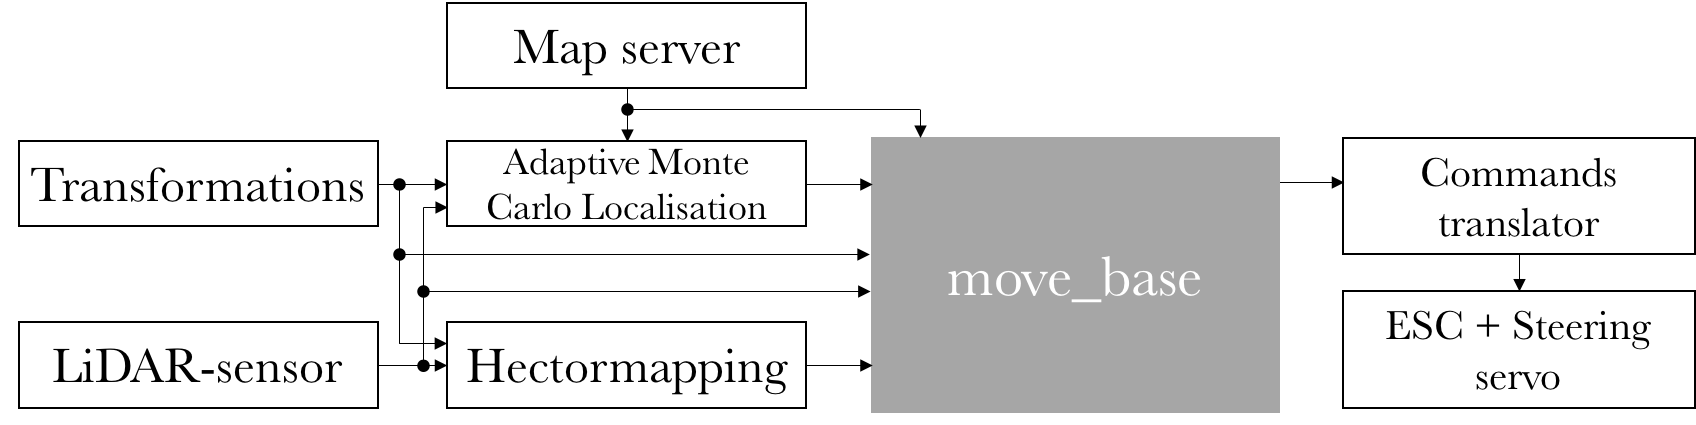
\includegraphics[width=\columnwidth]{navstack_overall}
	\centering
	\caption{Illustrates the integration of the \emph{move\textunderscore base}-node inside the existing environment}
	\label{fig:navstack_overall}
\end{figure}
\begin{figure}[!t]
	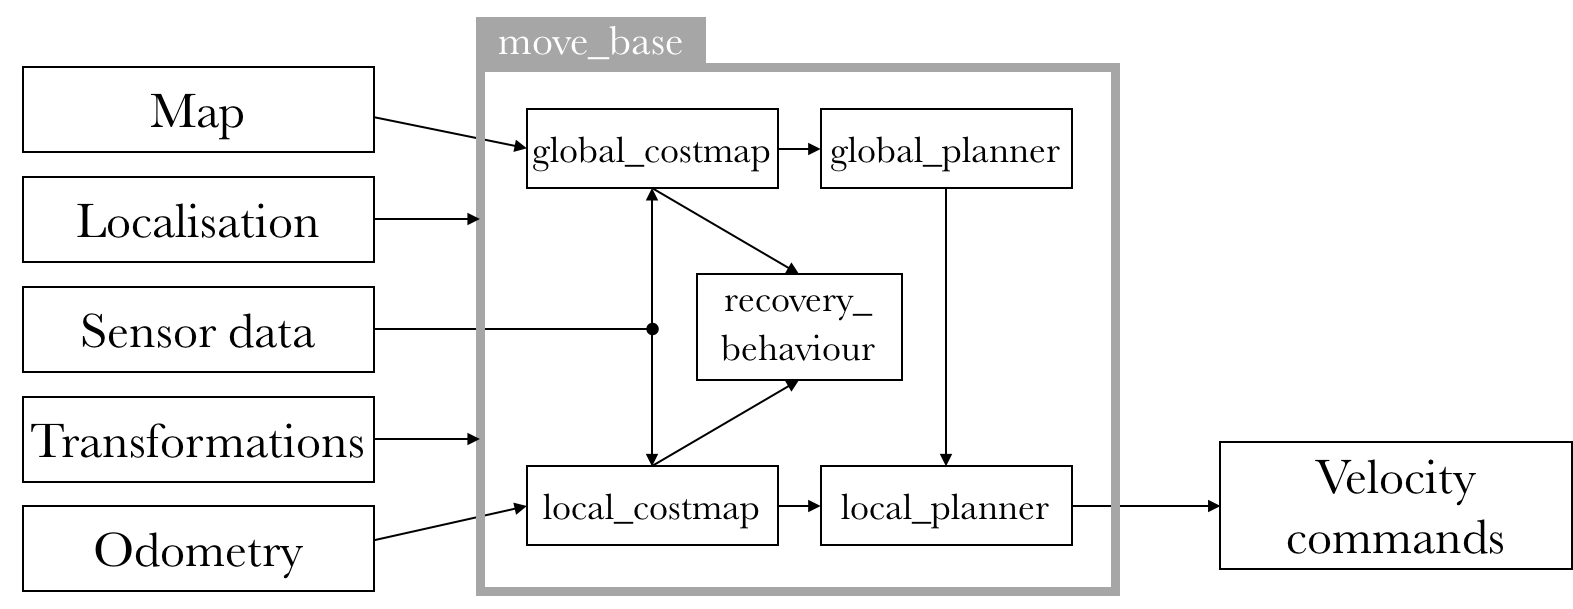
\includegraphics[width=\columnwidth]{navstack3}
	\centering
	\caption{Overview of the navigation stack with its input and output nodes, along with the plug-ins inside the \emph{move\textunderscore base}-node \cite{Marder-Eppstein2016}.}
	\label{fig:navstack_global}
\end{figure}

Inside the \textit{move\textunderscore base}-node, multiple calculations take place in order to navigate. 
\paragraph{Global Planning}
In order to make a global plan, a global costmap must be generated. This particular map is derived from the environment map, which in turn is made by \emph{hector\textunderscore mapping}. A costmap is an occupancy grid which specifies where the car is allowed to navigate. Another node named \emph{global\textunderscore planner} calculates a path from start to destination, using the global costmap. The default implementation of this planner is \emph{navfn}, which uses Dijkstra as path finding algorithm, but we opted for the more advanced planner \emph{global\textunderscore planner} because of the ability to customise multiple parameters. Unfortunately, the name of the implementation is the same as the one of the node, thus making the whole structure a bit unclear. 
\paragraph{Local Planning}
Second, the central node produces a local costmap which is used by the local planner. The costmap is made by obtaining LiDAR-information in a range of three meters around the car. In this way, unexpected obstacles are located on this costmap. Therefore, the local planner is able to plan a route around these obstructions. The default local planner is \emph{base\textunderscore local\textunderscore planner}\cite{Marder-Eppstein2017_2}. The planner is realised using Trajectory Rollout algorithm and Dynamic Window Approach\cite{Fox1997, Gerkey2008}. 
Though, another implementation is available for car-like robots. This planner is known as \emph{teb\textunderscore local\textunderscore planner} and it implements a methodology called \emph{timed elastic band}\cite{Rosmann2016}. As a safety feature, the \emph{move\textunderscore base}-node includes a recovery plug-in which plans a secondary route when the car is stuck and thus unable to follow the planned route.
Figure \ref{fig:navstack_global} shows an abstract overview of the navigation stack with its nodes and plug-ins \cite{Marder-Eppstein2016_2, Zheng2016}.


In order to use the \emph{move\textunderscore base}-node properly, certain precautions have to be made. First, the transformation tree has to be correct such that the laser data can be transformed to the center of the robot. To build such a tree, two transformation nodes are created. The first node transforms the LiDAR-data to a link that connects all types of sensors. The second node transforms the linking point to the center of the frame. Since only one sensor is present, we locate the linking point to the center of the frame; thus, the second transformation is one-to-one. Though, this second transform is needed as the navigation stack needs the \emph{base\textunderscore frame}-transformation \cite{Kohlbrecher2012_tf} \cite{Woodall2015}.

Second, the navigation stack needs a source of odometry data. Since the car does not feature a suitable source, we have to generate such data from the LiDAR-sensor. \emph{Hector\textunderscore mapping} has the ability to provide odometry data which is derived from the laser scan. By matching sequential scan frames, the occurred motion can be derived, which in turn can be outputted as odometry data. In order to use this odometry information in the navigation stack, a particular node is needed which translates the odometry information to transformation data. The implementation of this node is available on the \emph{f1tenth}-repository of Nischal K.N. \cite{K.N.2016}.

Third, the robot must be able to guess its location on the given map. This is implemented by the \emph{AMCL}-node (\emph{Adaptive Monte Carlo Localisation}). In order to generate a suitable pose guess, the node also needs odometry data, along with the map, transformations and LiDAR-information \cite{Gerkey2016} \cite{Thrun1999}. The pose guess is relative to the given map; thus, this node provides the transformation between the odometry and the map.\\
Final, the translation from the velocity commands of the navigator to instructions for the motor controller needs to be made.

\subsection{Waypoints}
A waypoint is similar to an instruction of  \emph{turn-by-turn}-based navigation. A waypoint consists of two datafields: \emph{direction} and \emph{count}.
The \emph{direction}-field has three possible options: \emph{straigt}, \emph{left} and \emph{right}. The \emph{count}-variable describes which turn should be taken. Figure \ref{fig:waypoints_turns} shows two examples. In the first case, the waypoint is described as $(\text{\emph{right}},\,2)$. I.e., the car should take the second exit on the right. The instruction of the second example is described as $(\text{\emph{left}},\,3)$. 

\begin{figure}[!t]
	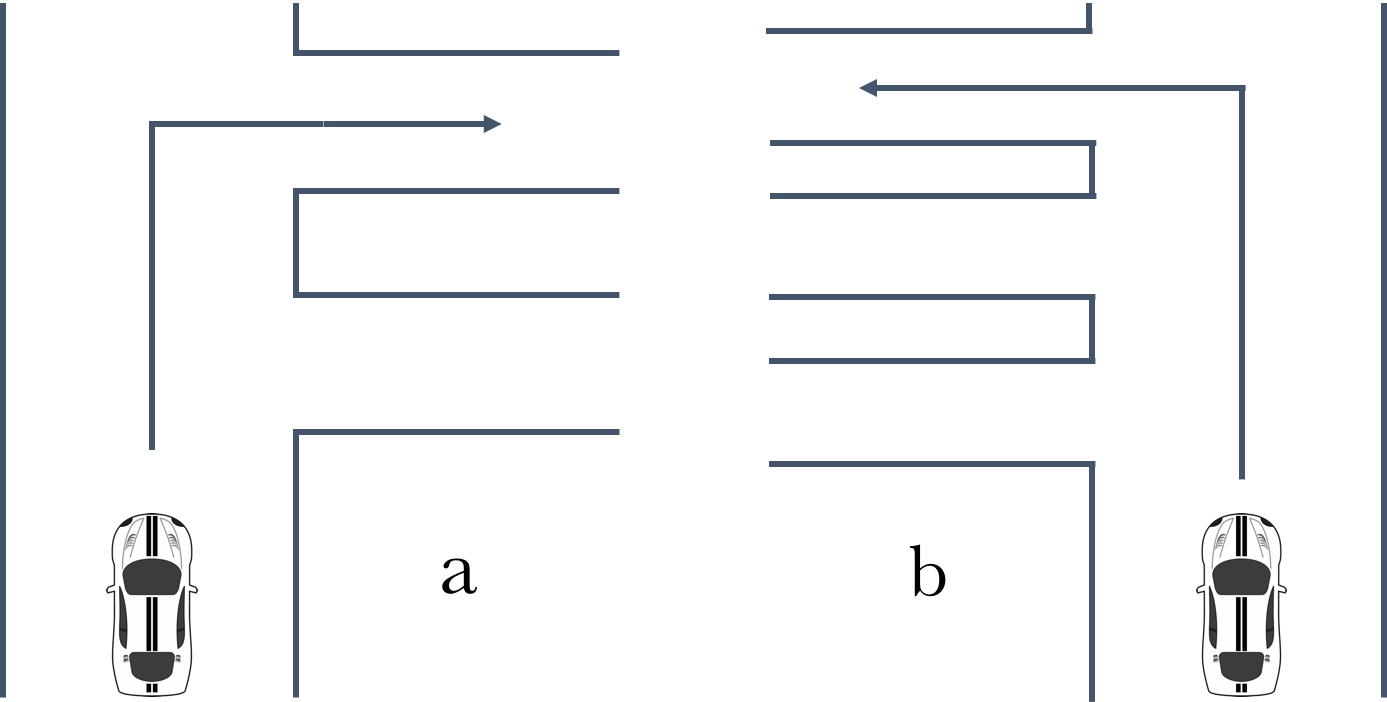
\includegraphics[width=\columnwidth]{waypoints_turns}
	\centering
	\caption{a) Illustrates a waypoint which is described as $(\text{\emph{right}},\,2)$. b) Shows the instruction $(\text{\emph{left}},\,3)$. }
	\label{fig:waypoints_turns}
\end{figure}

The following paragraph clarifies the algorithm. When the car is driving and detects a corner on one of its sides, the software checks if this is the corner that is specified by the waypoint instruction. If not, the car continues driving while setting the steering position to a neutral state, such that the car stays in the middle of the road. If the result is true, the car will take the turn by adjusting the wheel position until the car is parallel with the wall of the corner. When corners on both sides are detected, but neither of them is specified by the waypoint, the steering position is also set to neutral in order to keep driving straight until a wall on either side is detected.

The actual implementation of the algorithm is done by B. Smits and S. Maes for their bachelor's thesis \cite{SmitsMaes2017}. An elaborated discussion is found in their paper. It is also worth noting that we have to assume the car drives in the middle of the road. Smits and Maes implemented multiple ROS-nodes which adjust the wheel position of the car with given LiDAR-data, thus regulating the distance with respect to the wall while driving. 

\subsection{Optimisation Algorithm}
\label{sec:OptAlgorithm}
Due to the limited time frame of this thesis, the implementation of an optimisation algorithm has not finished yet. Though, as mentioned in the previous section, the Ferguson Splines used in \cite{Saska2006} are suitable for the F1/10-car.

\section{Test setup}
\label{sec:TestSetup}
\subsection{F1/10-car}
The car used in this research is driven by an NVIDIA Jetson TK1 development board. This board contains a System on a Chip (Soc), which is known as Tegra K1 from the same manufacturer. The SoC consists of a quad core CPU, which is made of four ARM Cortex-A15-cores. The CPU is assisted by 192 CUDA-cores as graphical unit.

The used operating system is an Ubuntu distribution, i.e. version 14.04. The ROS-ecosystem (Robot Operating System) serves as middleware application. This open-source framework provides different types of libraries and packages in order to develop custom robot applications. Different ROS-nodes communicate with each other via the Publish-Subscribe-methodology.

Additionally, multiple sensors are present. First, a Hokuyo UST-10LX serves as LiDAR-sensor on the robot. With a refresh rate of 40 Hz and an angle resolution of 0.25$\degree$ over a range of 270\degree, this sensor is capable of both fast and accurate measurements. Second, an IMU-sensor (Inertial Measurement Unit) is available. This sensor consists of a magnetometer, gyroscope and accelerometer, all of which have three axes, thus having nine degrees of freedom in total. The output of both of these sensors is handled by different ROS-nodes, which in turn publish the information to other nodes.

The body of the car itself is made by Traxxas. The Velineon VXL-3s serves as motor controller or ESC and is connected to a Teensy 3.2 development board, containing an ARM Cortex-M4 processor. The steering servo is also connected to this development board. The microcontroller generates two PWM-signals (Pulse Width Modulation) that are sent to the ESC and servo in order to control the behaviour of the car. This microcontroller also communicates with other nodes via ROS.

%The ESC (Electronic Speed Controller) and steering servo are connected to a Teensy 3.2 development board containing an ARM Cortex-M4 processor. This microcontroller generates two PWM-signals (Pulse Width Modulation) that are sent to the ESC and servo in order to control the behaviour of the car. This microcontroller also communicates with other nodes via ROS.

Figure \ref{fig:f1_lidar_tk1} shows the used LiDAR-sensor from Hokuyo and the NVIDIA Jetson TK1 development board.

\begin{figure}[!t]
	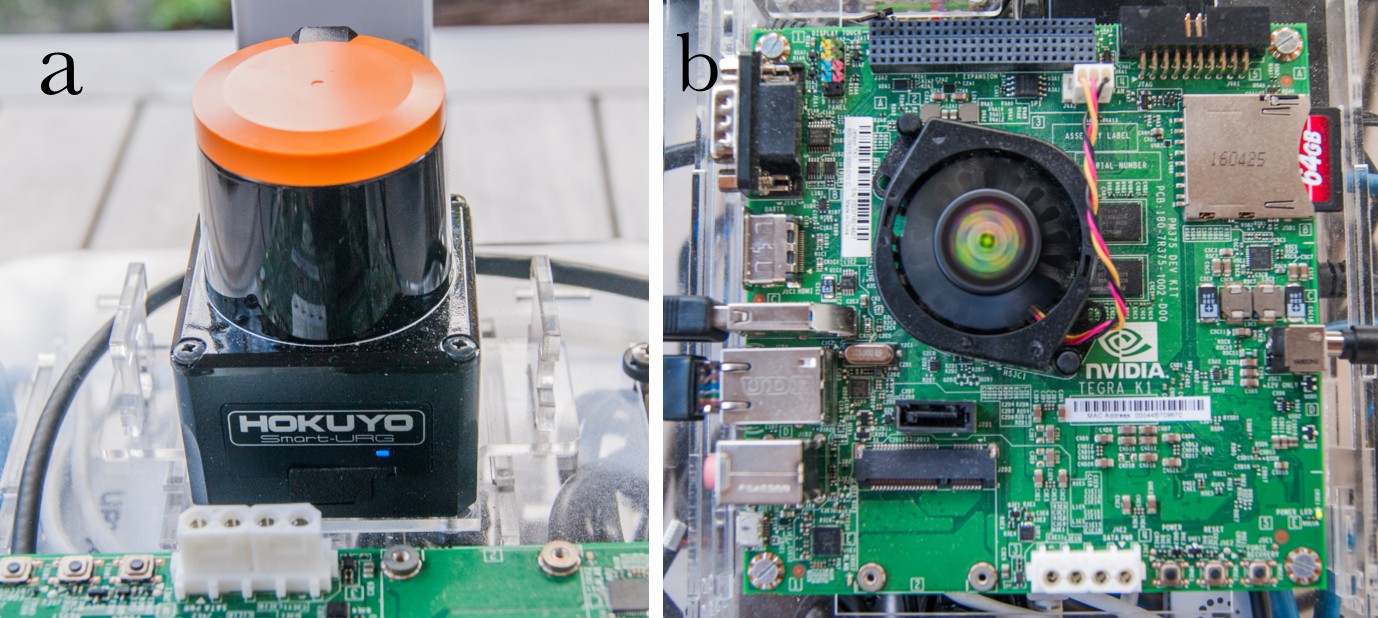
\includegraphics[width=\columnwidth]{f1_lidar_tk1}
	\centering
	\caption{a) Shows the Hokuyo UST-10LX as LiDAR-sensor. In b), the development board NVIDIA Jetson TK1 is shown.}
	\label{fig:f1_lidar_tk1}
\end{figure}

\subsection{Prerequisites}
Before the car was able to navigate in indoor environments, certain prerequisites had to be made. First, the car was unable to drive at a low speed. This low speed was needed to avoid heavy crashes when debugging the software. The general approach is to modulate the ESC-signal with a square wave, such that the motor controller is turned on and off, thus regulating the speed. The first solution was to modulate the signal with another PWM-signal. Thus, the duty cycle could be adjusted in order to regulate the motor power. Several problems arose when using this method. The speed controller does not accept high frequency signals with a low duty cycle. Additionally, the M4-processor could not generate block signals with a low frequency and high duty cycles.

Due to this problems, we were urged to develop a new solution. In this approach, the frequency varies while the duty cycle is fixed. For example, the motor has less time to accelerate when increasing frequency of the square wave. Obviously, the acceleration time increases as the frequency decreases, resulting in a smoother driving experience.

Another prerequisite we had to make, was the ability to drive at a constant speed. First, we opted for speed regulation via the IMU-sensor. Though, it appeared that this method was unable to derive the speed from the output data. We tried many methods such as a Kalman-filter, complementary filter or derivation of speed from raw accelerometer data, but all of the obtained resuls were not as expected. Therefore, an RPM-sensor from Traxxas is integrated in the body and is connected to the Teensy development board. The sensor is based on the Reed-principle. Every 100 ms, the Teensy board counts how many rotations occurred. This value is published via ROS. A speed regulator, which uses this RPM-counter, is implemented in the bachelor's thesis of Smits and Maes \cite{SmitsMaes2017}.

\section{Results}
\label{sec:Results}
\subsection{Fixed Path}
The navigation stack is installed on the NVIDIA Jetson. In order to control this navigator, we utilised an external virtual machine (VM) running Ubuntu 16.04. This VM provides the \emph{rviz}-environment, which is a visualisation tool in ROS. Using this tool, we are able to send locations to the navigation stack, such as pose estimates and goals. These locations are specified by a position in the XYZ-space and a quaternion as orientation. The units are respectively meters and radians. When using the navigation stack, the \emph{rviz}-tool visualises the position of the car, the calculated paths and the provided map. This visualisation is shown in figure \ref{fig:navstack_result}.
Figure \ref{fig:navstack_tf} illustrates the transformations which are created by the transformation nodes of the navigation stack.

\begin{figure}[!t]
	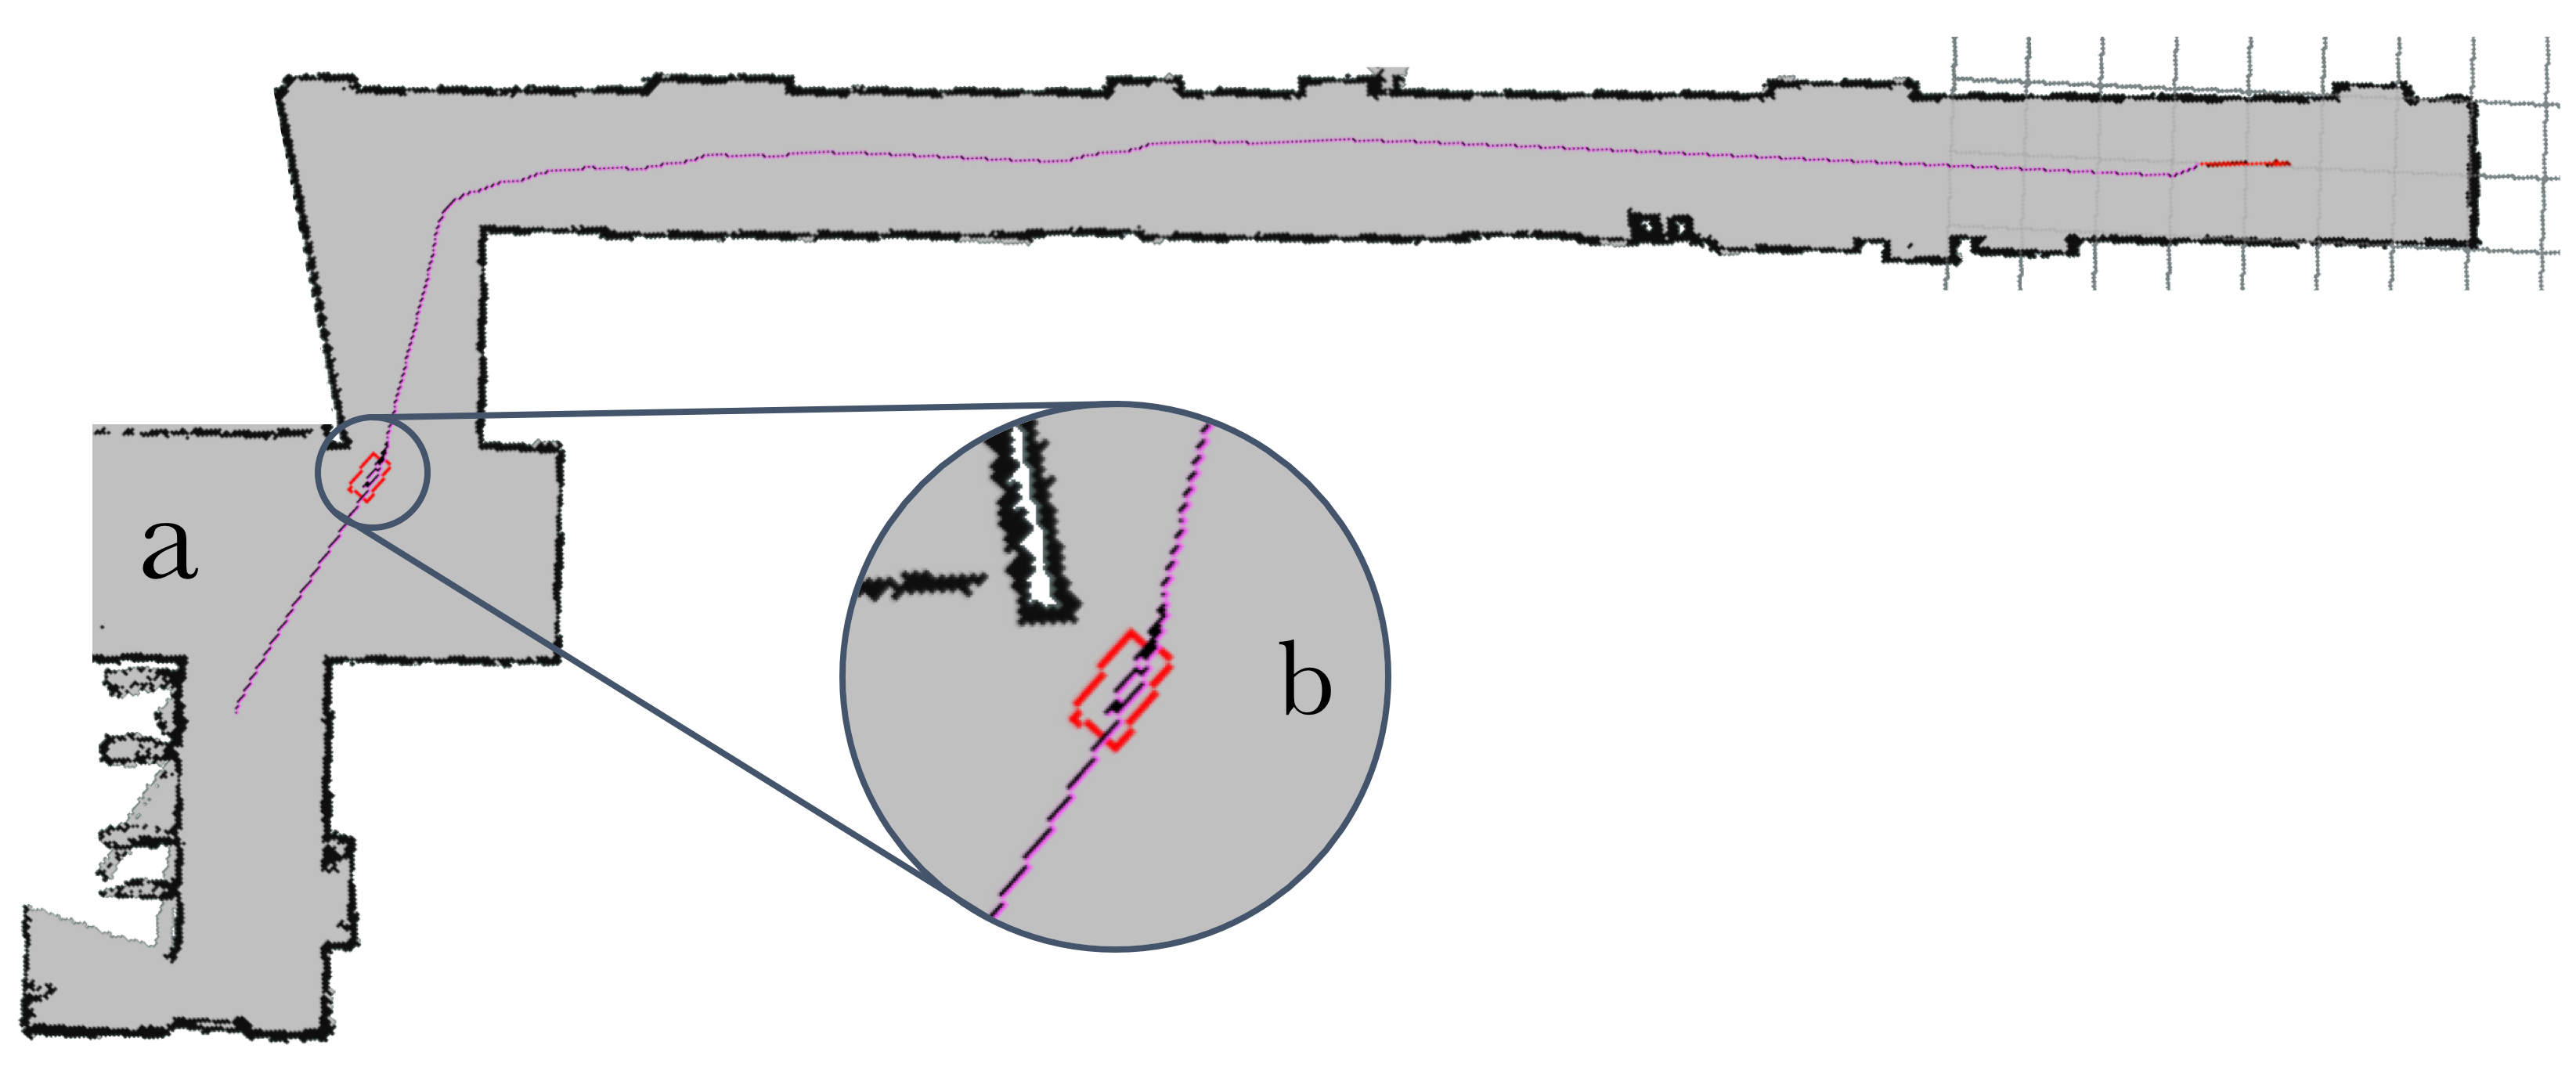
\includegraphics[width=\columnwidth]{navstack_result_1}
	\centering
	\caption{a) shows the route which is planned by the navigation stack. The map is built with \emph{hector\textunderscore mapping}\cite{Kohlbrecher2012}. b) illustrates a close-up of the car moving on the route. }
	\label{fig:navstack_result}
\end{figure}

\begin{figure}[!t]
	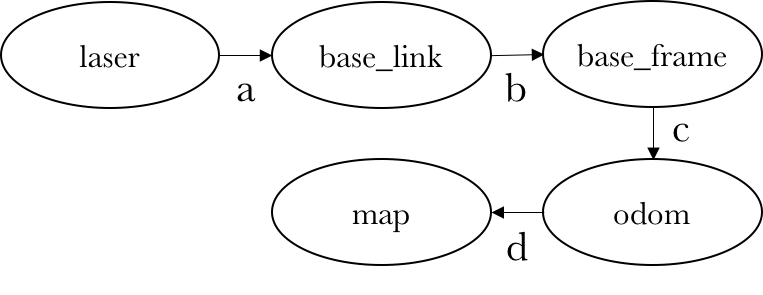
\includegraphics[width=\columnwidth]{navstack_tf2}
	\centering
	\caption{Created transformation frames for the navigation stack. a) and b) are static transformations. The transformation in c) is provided using the odometry data from \emph{hector\textunderscore mapping}. d) is provided by the \emph{AMCL}-node, which links the map with the pose of the robot.}
	\label{fig:navstack_tf}
\end{figure}

A major drawback of the navigation stack is its lack of optimisation for car-like robots. Instead, it is especially created for robots with holonomic or differential steering mechanisms. Therefore, the car is sometimes unable to follow the calculated path. Because of this problem, we implemented \emph{teb\textunderscore local\textunderscore planner} such that the route would be more optimised for Ackermann-steering. It appeared that this planner needed a lot of computing power. The onboard NVIDIA Jetson TK1 was unable to calculate paths at a requested rate of 2 Hz. Instead, each calculation lasted approximately three seconds. Even a virtual machine with high specifications was unable to meet the requirements. The virtual machine was hosted by a macOS-host with Parallels as virtualisation software. The specifications were set to eight virtual cores and four gigabytes of RAM. Because of this latency, the default local planner was used for further usage. Although using this planner could result in pivot points and sharp curves, the car is perfectly able to navigate on the trajectory if the curves are almost straight and without turning points.
Another limitation is the low driving speed at which the car has to drive in order to update its position. By increasing speed, a certain latency exists between the actual position and the calculated one. As a result, the navigation stack is too slow with processing a new local path, so crashes could occur.

A final adjustment is made in the goal tolerance. Because of the Ackermann-steering mechanism, chances are that the goal is never reached due to the constraints of a car-like robot. To overcome this problem, a certain tolerance is set for both position and orientation. A margin of one meter is set for the position, whereas an orientation margin of $2\pi$ is active such that any orientation is possible in order to reach the goal.

\subsection{Waypoints}
With the first implementation of the waypoints algorithm, the system detected many false positives. That is, the car turned left or right while a corner was absent. This phenomenon happened when, for example, the car was in the vicinity of a door. After a few adjustments, the detection rate of false positives decreased drastically. 

A major drawback of this algorithm is the use of raw LiDAR-data. When the car is driving along a black object, the laser beam does not return a reflection, which results in the maximum range of the sensor. Thus, the algorithm detects a corner and the car starts to manoeuvre. This problem is partially solved by taking multiple measurements on different angles. However, the problem still occurs when using large black objects. Though, none of these problems occur in environments without black objects. 

An advantage of this method is the ability to maintain a high speed. By relying on raw LiDAR-data instead of location tracking, the refresh rate of the algorithm is much higher. 

\subsection{Optimisation Algorithm}
As mentioned in section \ref{sec:OptAlgorithm}, no implementation and results are available yet. Though, we expect that parameter optimisations are needed and many iterations of the PSO-algorithm are required in order to navigate the car using the calculated paths.

\section{Comparative study}
\label{sec:ComparativeStudy}
The first method was to navigate on a fixed path. Using this method, an accurate destination can be reached as it is specified in very precise values. Though, a tolerance is set in order to reach the goal properly with a car-like robot. In case of a holonomic robot or a robot with a differential steering mechanism, this tolerance is not required. A drawback of this navigation stack is the slow refresh rate. Therefore, only low speeds are possible. If a faster speed is applied, the module is unable to keep up with the fast location updates. These advantages and disadvantages make this approach suitable for applications where a low speed is not really a drawback, but an exact destination is required.

The second algorithm, on the other hand, is capable of maintaining high speeds as no location tracking is needed. As mentioned in the previous section, the refresh rate of this algorithm is much higher. Each time the LiDAR-sensor publishes a message, the algorithm is executed. Hence, the refresh rate is 40 Hz. A drawback of this methodology is the inaccuracy of the goal. The algorithm is not capable of reaching an exact destination point. Instead, the goal is an abstract instruction. This waypoint approach is suitable for applications where the maximum speed is really important and the destination point does not need to be exact. An example of such an application is an indoor race track with many possible passages.

According to \cite{Saska2006}, the optimisation algorithm is able to calculate a path for a car-like robot in a complex environment. Though, a real-time update of the path is not possible yet without restarting the algorithm. 

\section{Further Research}
\label{sec:FurtherResearch}
First of all, the optimisation algorithm, developed by Saska \cite{Saska2006}, needs to be implemented and compared to the other algorithms in order to finish the research. 

As mentioned in the previous paragraph, the algorithm of Saska has a slow update speed. However, if we are able to combine the work of Saska with the algorithm of Nasrollahy \cite{Nasrollahy2009}, which suggests a PSO-method for using in a dynamically changing environment, then we have path planner for car-like robots which updates in real-time. This would be an advantage in comparison with the navigation stack of our first method. The only drawback would be the location tracking. Therefore, only a low speed can be maintained. 

By optimising the location tracker, which is used in the navigation stack and the optimisation algorithm, we are able to increase the update rate, thus resulting in a higher maximum driving speed.

Additionally, research could be conducted in optimising the navigation stack for car-like robots. 

\section{Conclusion}
\label{sec:Conclusion}
In order to explore the navigation capabilities of an F1/10-car, this paper has introduced three different types of navigation algorithms. I.e., navigating by a fixed path, via waypoint instructions and via an optimisation algorithm. The paper implemented two algorithms instead of three, due to the limited time frame. These two algorithms have been compared with each other. The drawback of the first method is the limit to low driving speeds, while the accurate specification of a goal makes the algorithm suitable for exact navigation commands. The second algorithm is able to maintain higher speeds, but a goal is specified in a more abstract way. Thus, the algorithm is ideal in environments where speed is more important than the goal.
The last algorithm is listed in further research, as it needs to be implemented and tested to finish the research.


% trigger a \newpage just before the given reference
% number - used to balance the columns on the last page
% adjust value as needed - may need to be readjusted if
% the document is modified later
%\IEEEtriggeratref{8}
% The "triggered" command can be changed if desired:
%\IEEEtriggercmd{\enlargethispage{-5in}}

% references section

% can use a bibliography generated by BibTeX as a .bbl file
% BibTeX documentation can be easily obtained at:
% http://www.ctan.org/tex-archive/biblio/bibtex/contrib/doc/
% The IEEEtran BibTeX style support page is at:
% http://www.michaelshell.org/tex/ieeetran/bibtex/
%\bibliographystyle{IEEEtran}
% argument is your BibTeX string definitions and bibliography database(s)
%\bibliography{IEEEabrv,../bib/paper}
%
% <OR> manually copy in the resultant .bbl file
% set second argument of \begin to the number of references
% (used to reserve space for the reference number labels box)

%\begin{thebibliography}{1}

%\bibitem{IEEEhowto:kopka}
%H.~Kopka and P.~W. Daly, \emph{A Guide to \LaTeX}, 3rd~ed.\hskip 1em plus
%  0.5em minus 0.4em\relax Harlow, England: Addison-Wesley, 1999.

%\end{thebibliography}
\newpage
\bibliographystyle{plain}
\bibliography{bibliography.bib}
%\bibliography{bibliography.bib}




% that's all folks
\end{document}